\documentclass[conference]{IEEEtran}
\usepackage{graphicx}
\usepackage{booktabs}
\usepackage{amsmath}
\usepackage{cite}
\usepackage{url}

% balanced multi-row author block (standard IEEE template helper)
\makeatletter
\newcommand{\linebreakand}{%
  \end{@IEEEauthorhalign}\hfill\mbox{}\par
  \mbox{}\hfill\begin{@IEEEauthorhalign}
}
\makeatother

\begin{document}

\title{PhysioTwin: Teaching, Verifying, and Grading Robotic Rehabilitation
Exercises with a Single Consumer Smartwatch}

\author{
\IEEEauthorblockN{Firaol Tesfaye}
\IEEEauthorblockA{Higher Colleges of Technology\\
Dubai, UAE\\
h00539876@hct.ac.ae}
\and
\IEEEauthorblockN{Milki Teshome}
\IEEEauthorblockA{Higher Colleges of Technology\\
Dubai, UAE\\
h00539899@hct.ac.ae}
\linebreakand
\IEEEauthorblockN{Moez Rehman}
\IEEEauthorblockA{Higher Colleges of Technology\\
Dubai, UAE\\
mrehman1@hct.ac.ae}
\and
\IEEEauthorblockN{Yassine Benachour}
\IEEEauthorblockA{Higher Colleges of Technology\\
Dubai, UAE\\
ybenachour@hct.ac.ae}
}

\maketitle

\begin{abstract}
Robot-assisted therapy can guide an impaired upper limb through
prescribed exercises, but programming patient-specific trajectories
today requires motion-capture laboratories or hands-on kinesthetic
teaching. We present PhysioTwin, a pipeline in which a single consumer
smartwatch is the entire interface to a rehabilitation robot: a
demonstration recorded on the wrist teaches the robot an exercise, and
the same sensing pipeline later verifies and grades performance. The
system builds on a new dataset of 240 sessions from 11 healthy
subjects performing 12 prescribed upper-limb exercises, most recorded
simultaneously on both wrists. With it we provide the first
ground-truth validation of the bilateral mirror-symmetry assumption;
expose a severe cross-wrist deployment gap in exercise recognition and
close it with a data-certified mirror transformation; learn exercises
as dynamic movement primitives and execute them on a
\emph{physics-simulated} UR5e; close the loop by recognizing the
simulated robot's executions through a virtual watch; and grade
movement quality against population and personalized motion envelopes.
Subject-independent recognition exceeds 92\%, and mirror-aware
training restores cross-wrist accuracy to statistical equivalence with
the within-wrist level. All
experiments are reproducible from the accompanying repository.
\end{abstract}

\begin{IEEEkeywords}
rehabilitation robotics, wearable sensors, smartwatch, learning from
demonstration, dynamic movement primitives, human activity recognition
\end{IEEEkeywords}

\section{Introduction}
Musculoskeletal disorders of the shoulder, elbow, and wrist are among
the most common reasons for physiotherapy referral, and their
treatment depends on patients performing prescribed exercises
correctly and consistently at home. Adherence is notoriously poor and
largely invisible to the clinician: between appointments, therapists
typically rely on patient self-reports. Two technology families
address parts of this problem. Wearable-sensor systems can recognize
and count exercises from a wrist-worn inertial measurement unit
(IMU)~\cite{burns2018}, giving clinicians objective adherence data ---
a rapidly growing field surveyed in~\cite{benachour2026review}.
Rehabilitation robots can physically guide an impaired limb through
its prescribed motion with assist-as-needed
control~\cite{krebs1998,maciejasz2014}, taking over the repetitive
guidance work of the therapist. The two families, however, have remained separate:
the robots are programmed through motion-capture laboratories,
teach-pendant programming, or hands-on kinesthetic teaching --- all of
which require the therapist and the robot to share a room and
specialized equipment.

This paper connects the two families with the cheapest sensor a
patient already owns. In the proposed pipeline, which we call
\emph{PhysioTwin}, a demonstration of a prescribed exercise ---
recorded by an ordinary smartwatch on the demonstrator's wrist,
anywhere --- is converted into a robot-executable motion primitive.
A compliant robot arm can then guide the patient's limb through that
exercise; the clinical motivation follows mirror
therapy~\cite{ramachandran1996,thieme2018}, in which the movement of
the unaffected limb serves as the template for the affected one. The
same smartwatch pipeline subsequently \emph{verifies} what was
executed and \emph{grades} its quality. One consumer device is thus
the robot's teacher, the exercise's examiner, and the patient's
monitor.

The work is grounded in a new dual-wrist dataset (Section~III) whose
distinguishing property is simultaneity: subjects performed bilateral
exercises wearing a watch on each wrist, so almost every left-wrist
recording has a synchronized right-wrist counterpart (107 of 109
pairs). This enables experiments
that were previously impossible, most importantly a ground-truth test
of the mirror-symmetry assumption that underlies both mirror therapy
instrumentation and left/right data augmentation in wearable machine
learning.

The contributions are:
\begin{enumerate}
\item the first ground-truth validation of bilateral mirror symmetry
from synchronized dual-wrist consumer smartwatches, quantified per
exercise (Section~V-A);
\item the first measurement of the cross-wrist deployment gap for
clinical exercise recognition (a 33--40 percentage-point collapse
against the within-wrist reference) and
its closure with a data-certified mirror transformation --- to
statistical equivalence with within-wrist recognition, evaluated under
the strictest unseen-subject-and-unseen-wrist protocol
(Section~V-B);
\item an end-to-end, reproducible pipeline from smartwatch
demonstration to robot execution --- repetition segmentation, dynamic
movement primitive (DMP) learning, kinematic retargeting to a UR5e,
and physics-simulated execution through the standard ROS~2 control
stack (Sections~V-C, V-D);
\item a closed verification loop in which a classifier trained
exclusively on human recordings recognizes the robot's executions
through a virtual watch (Section~V-E); and
\item a movement-quality grading scheme based on population and
personalized motion envelopes, evaluated on 2{,}452 genuine
repetitions with controlled fault injection (Section~V-F).
\end{enumerate}

All experiments are healthy-subject and simulation-based by design;
Section~VI discusses this scope honestly.

\section{Related Work}
\textbf{Wearable exercise recognition.} Burns
et~al.~\cite{burns2018} established smartwatch-based recognition of
shoulder physiotherapy exercises; subsequent work has raised accuracy
with deep models and larger exercise vocabularies. Feature-engineered
classical pipelines remain competitive at small subject counts; the
present dataset's pilot predecessor was analyzed this way by Benachour
et~al.~\cite{benachour2025}, who optimized windowing, feature
selection, and classical models on three movements from three
subjects. Follow-up studies from the same group compared classical
models and an RNN for wearable rehabilitation movement classification
and examined their on-device deployment feasibility~\cite{araya2025},
and proposed a hybrid CNN--LSTM that, notably, closed its
subject-independent generalization gap by fine-tuning on roughly 60~s
of user calibration data~\cite{eshetu2026} --- independently
corroborating the value of short calibration sessions that our
personalized quality envelope exploits (Section~V-F). Parallel work in
the group explores dynamic-time-warping representations for upper-limb
IMU classification --- combinatorial DTW medoid
distances~\cite{kedir2026} and prototype-based DTW
features~\cite{bona2026} --- an alternative movement-representation
route to the windowed statistical features used here. We adopt this
line's windowing/feature philosophy for our recognition baseline but
address questions that require the new dataset's scale and dual-wrist
design.

\textbf{Sensor placement and the wearing-side problem.} Cross-position
generalization is a recognized open problem in human activity
recognition~\cite{bulling2014}. For the specific left/right wrist
question, prior work has simulated the opposite wrist by mirroring
signal axes; to our knowledge no public dataset provides synchronized
recordings of the same movement from both wrists, so the mirror
assumption itself has not previously been testable.

\textbf{Robot-assisted upper-limb therapy.} From the pioneering
MIT-MANUS trials~\cite{krebs1998} to today's end-effector and
exoskeleton devices~\cite{maciejasz2014}, robot-assisted upper-limb
therapy is clinically established, and assist-as-needed control is
standard. Exercise content, however, is programmed through
preinstalled libraries, kinesthetic teaching, or motion capture.
Learning from demonstration~\cite{argall2009}, notably with
DMPs~\cite{ijspeert2013}, is a mature robotics technique, and
IMU-driven demonstration has been explored for reaching motions; a
consumer smartwatch as the sole teaching interface for rehabilitation
exercises has not been reported.

\textbf{Mirror therapy.} Using the healthy limb's motion as the
template for the impaired one has clinical foundations in mirror-box
therapy~\cite{ramachandran1996} and meta-analytic support in
stroke rehabilitation~\cite{thieme2018}. PhysioTwin can be read as a
robotic instantiation: the healthy arm demonstrates, the robot
reproduces the mirrored motion on the affected side.

\textbf{Movement quality.} Smoothness metrics, notably log
dimensionless jerk~\cite{balasubramanian2015}, are validated proxies
of motor performance. Learned anomaly detectors have also been applied
to rehabilitation monitoring --- e.g., a hybrid multi-task LSTM
autoencoder for semantic anomaly diagnosis~\cite{benachour2026ae} ---
whereas we deliberately choose interpretable per-repetition envelopes
(range, tempo, spectral, and end-point features), whose individual
bounds name the fault they flag; the two approaches are complementary.

\section{Dataset}

\subsection{Participants and ethics}
Eleven healthy university-student volunteers (anonymized S01--S11) took
part, aged 20--24 years, of mixed gender and predominantly
right-handed. Inclusion required no current upper-limb injury, pain, or
movement restriction; no affected limb or movement constraint was
observed for any participant, and all recordings are labelled as
performed with unaffected limbs. Every volunteer completed and signed a
written informed-consent form prior to data collection, and the study
was conducted under approval from the Higher Colleges of Technology
research ethics committee. Participant identities are anonymized
throughout the released code and results. A dedicated companion paper
will report the full participant, protocol, and data-collection
methodology in detail; here we summarize only what is needed to
interpret the experiments.

\subsection{Acquisition setup}
Recordings were made with two Apple Watch units (watchOS
26.2--26.3) running a custom watchOS acquisition application; the
\emph{same two physical devices} were used for all subjects, one
always on the left wrist with the crown facing right and the other
always on the right wrist with the crown facing left (watch face
dorsal, standard wear). Each session logs the CoreMotion device-motion
service at a nominal 100~Hz: attitude quaternion in the
\texttt{XArbitraryCorrectedZVertical} reference frame (gravity-aligned
$z$, arbitrary heading), rotation rate (rad/s), user acceleration and
gravity (units of $g$), alongside the raw accelerometer stream and a
per-session metadata file. No user-side calibration is performed
beyond CoreMotion's internal sensor fusion. Every sample carries a
Unix-epoch millisecond timestamp from the watch's NTP-disciplined
clock, which synchronizes the two devices; residual offset is absorbed
in analysis by a $\pm1$~s cross-correlation lag search. Effective
sampling rates span 99.5--100.2~Hz, and sample delivery is 99.86\%
complete: 1{,}497 of 1.09~million expected samples are absent as brief
dropouts (largest single gap 163~ms), which the common-grid resampling
of Section~IV-A absorbs.

\subsection{Exercise protocol}
Each subject performed 12 prescribed upper-limb rehabilitation
exercises associated with seven musculoskeletal conditions (e.g.,
frozen shoulder, shoulder impingement, distal radius fracture): bicep
curl, external rotation, forearm pronation--supination, front and
lateral deltoid raises, scaption, scapular retraction, ulnar nerve
glide, wand flexion, wand extension, banded overhead reach, and
one-arm tricep extension. All subjects followed the same protocol:
continuous self-paced repetitions for a fixed per-exercise recording
duration (30~s for the wand exercises, 90~s for the ulnar nerve
glide, 40~s otherwise), yielding a median of 10 repetitions per
session with no rest periods within a session. Participants received
in-person training on the purpose and use of the recording application
and a live demonstration of the exercises, and were additionally given
a detailed video tutorial (application manual, recording and sharing
steps, best-practice guidance, and clips of all 12 exercises) enabling
independent collection; participants recorded in pairs, each
checking the other's setup and execution, to ensure data validity. This gives 240 analysed sessions and roughly 3.0~hours
of motion. The property
central to this paper is that ten of the twelve exercises were
performed \emph{bilaterally with a watch on each wrist}: of 109
left/right session pairs, 107 overlap in absolute time --- synchronized
recordings of the same physical movement seen from both wrists (the
remaining two --- banded overhead reach and one-arm tricep extension
--- are single-arm by design). A complete protocol would give 242
sessions and 110 pairs: three recordings are absent and one exercise
was recorded twice, giving 240 sessions, and because one of the absent
recordings is the left-wrist half of a bilateral session there are 109
pairs rather than 110. Nothing was excluded from analysis.

\section{Methods}

\subsection{Frame-invariant motion representation}
The two watches occupy different body frames (opposite wrists,
opposite crown orientations), and each device-motion stream has an
arbitrary heading reference. All cross-wrist comparisons therefore use
quantities invariant to the sensor frame. From the attitude
quaternion sequence $q(t)$, resampled onto a common 100~Hz grid by
spherical linear interpolation, we compute the rotation angle relative
to the session's initial pose,
$\theta(t) = \angle\!\left(q_{\mathrm{ref}}^{-1} q(t)\right)$,
and the angular speed $\|\omega(t)\|$ from the gyroscope. Residual
clock offset between watches is absorbed by a $\pm 1$~s lag search.

\subsection{Mirror validation}
For each synchronized left/right pair we correlate the two wrists'
$\theta(t)$ profiles (Pearson $r$, after lag alignment) and report the
RMSE in degrees. Because $\theta(t)$ is frame-invariant, agreement
directly measures bilateral \emph{motion} symmetry rather than sensor
alignment. Note what this does and does not establish: $\theta(t)$ is
a rotation \emph{magnitude}, so agreement between the two wrists
validates that the arms traverse the same angular excursion with the
same timing --- the amplitude and phase of the movement. It does not
by itself establish the signed, axis-by-axis reflection relating the
two sensor frames; that is the separate object estimated as the mirror
map in Section~IV-C. The two are complementary: the magnitude result
says the arms genuinely move alike, and the sign map says how their
measurements relate.

\subsection{Exercise recognition and the mirror map}
Recognition follows the standard windowing pipeline: 2.56~s windows
with 50\% overlap; per window, 12 time- and frequency-domain
statistics for each of 13 channels (user acceleration, rotation rate,
gravity, pitch, roll, and the two frame-invariant magnitudes), for 156
features; a 300-tree random forest; and strict leave-one-subject-out
(LOSO) evaluation for the within-wrist baseline. Absolute yaw is excluded because its arbitrary
per-session reference would leak session identity. Session-level
decisions use majority voting. Two evaluation protocols are used for
cross-wrist transfer and should not be confused. The first holds out
the \emph{wrist} but not the subject: it trains on one wrist's
recordings from all subjects and tests on the other wrist. The second,
used for every
deployment-relevant claim, holds out \emph{both} --- the test subject
and the test wrist are unseen.

For cross-wrist transfer we estimate a \emph{data-certified mirror
map}: for every channel, the sign relating left- and right-wrist
signals is taken as the sign of the median correlation across the
synchronized pairs. Training data are then mirrored through this map
(alone or as augmentation), and evaluation includes the strictest
protocol in which the test subject \emph{and} the test wrist are both
unseen. To rule out leakage through the transformation itself, the
map was re-estimated within every LOSO training fold (i.e., excluding
the held-out subject's pairs): the resulting sign patterns are
identical to the global map in all 11 folds, so no information from
the test subject enters the mirror transformation. No other
preprocessing uses dataset-level statistics --- features are computed
per window, and random-forest training requires no global
normalization.

To ask whether mirror-augmented cross-wrist recognition is
\emph{equivalent} to within-wrist recognition rather than merely not
significantly different from it, both arms are evaluated on the same
held-out subject and the same test-wrist windows, giving 22 paired
folds (11 subjects $\times$ 2 transfer directions). We report a paired
Wilcoxon signed-rank test of difference and, because equivalence is
the claim of interest, two one-sided tests (TOST) against a
pre-specified margin of 2 accuracy points.

\subsection{Repetition segmentation and primitive learning}
Repetitions are segmented from the smoothed $\theta(t)$ profile by
peak detection (prominence 40\% of range) with boundaries at
inter-peak minima. Each session's median-duration repetition serves as
the demonstration and is encoded as a discrete
DMP~\cite{ijspeert2013} (50 radial basis functions per dimension) on
the heading-normalized rotation vector. DMP time and goal parameters
provide the clinically required scaling knobs: tempo ($\tau$) and
range of motion (goal).

\subsection{Retargeting and execution}
The robot reproduces the \emph{hand path} rather than imitating human
anatomy: a virtual elbow is anchored a forearm's length (0.25~m) above
the UR5e's home tool pose, and the tool tracks
$p(t) = a + R(t)\,v_0$, $R_{\mathrm{tool}}(t) = R(t)\,R_0$, where
$R(t)$ is the demonstrated wrist rotation re-referenced to the
repetition start. Joint trajectories are obtained by damped
least-squares inverse kinematics with singularity-adaptive damping and
step capping, checked against UR5e joint and speed limits, and
executed in Gazebo through the ROS~2
\texttt{joint\_trajectory\_controller} as five-repetition therapy sets
with 2~s return-to-start blends, at therapy pace (at least half the
demonstration speed, slower where speed limits require).

\subsection{Virtual-watch verification and quality grading}
A virtual watch is strapped to the executed motion: from recorded
joint states, forward kinematics reconstructs the tool rotation, which
is re-expressed in the demonstrating watch's frame (composing the
session reference and repetition-start attitudes) and
speed-compensated back to demonstration tempo; gravity, rotation rate,
user acceleration, pitch, and roll are then synthesized and passed
through the unchanged recognition pipeline.

Quality grading summarizes each repetition by six interpretable
features: range of motion, active duration, range-normalized peak
speed, log dimensionless jerk~\cite{balasubramanian2015},
high-frequency ($>$3~Hz) velocity power, and end-point
(return-to-start) error. An exercise's \emph{envelope} is a robust
interval (median $\pm K\cdot$MAD, per-feature $K$) learned from
genuine repetitions; bounds are one-sided where only one direction is
clinically abnormal. Faults are injected into genuine human
repetitions --- 2$\times$ speed, half range, 4~Hz/3$^{\circ}$ tremor,
truncation at 60\% --- and detection is evaluated LOSO. A
\emph{personalized} envelope centers the intervals on a subject's own
calibration repetitions (every second repetition) with the population
width as a floor. Operationally this corresponds to a brief supervised
calibration --- a handful of correctly performed repetitions recorded
under clinician observation at the start of a treatment block --- after
which unsupervised home sessions are graded against that patient's own
baseline; the population floor guards against the small calibration set
under-estimating natural variability.

\section{Results}

\subsection{Bilateral mirror symmetry (Experiment 1)}
Across 107 synchronized pairs, 9 of 10 dual-wrist exercises show
left/right rotation-profile correlations of $r \ge 0.97$ (most
0.99--1.00) with 4--16$^{\circ}$ RMSE (Fig.~\ref{fig:exp1}). External
rotation is the outlier ($r = 0.75 \pm 0.16$): its rotation amplitude
is small ($\approx 40^{\circ}$ versus up to $170^{\circ}$ for curls)
and genuine inter-arm asymmetry is visible in the profiles. Bilateral
mirror symmetry --- previously an assumption --- is thus quantified:
excellent for gross exercises, measurably imperfect for subtle ones.

\begin{figure}[t]
\centering
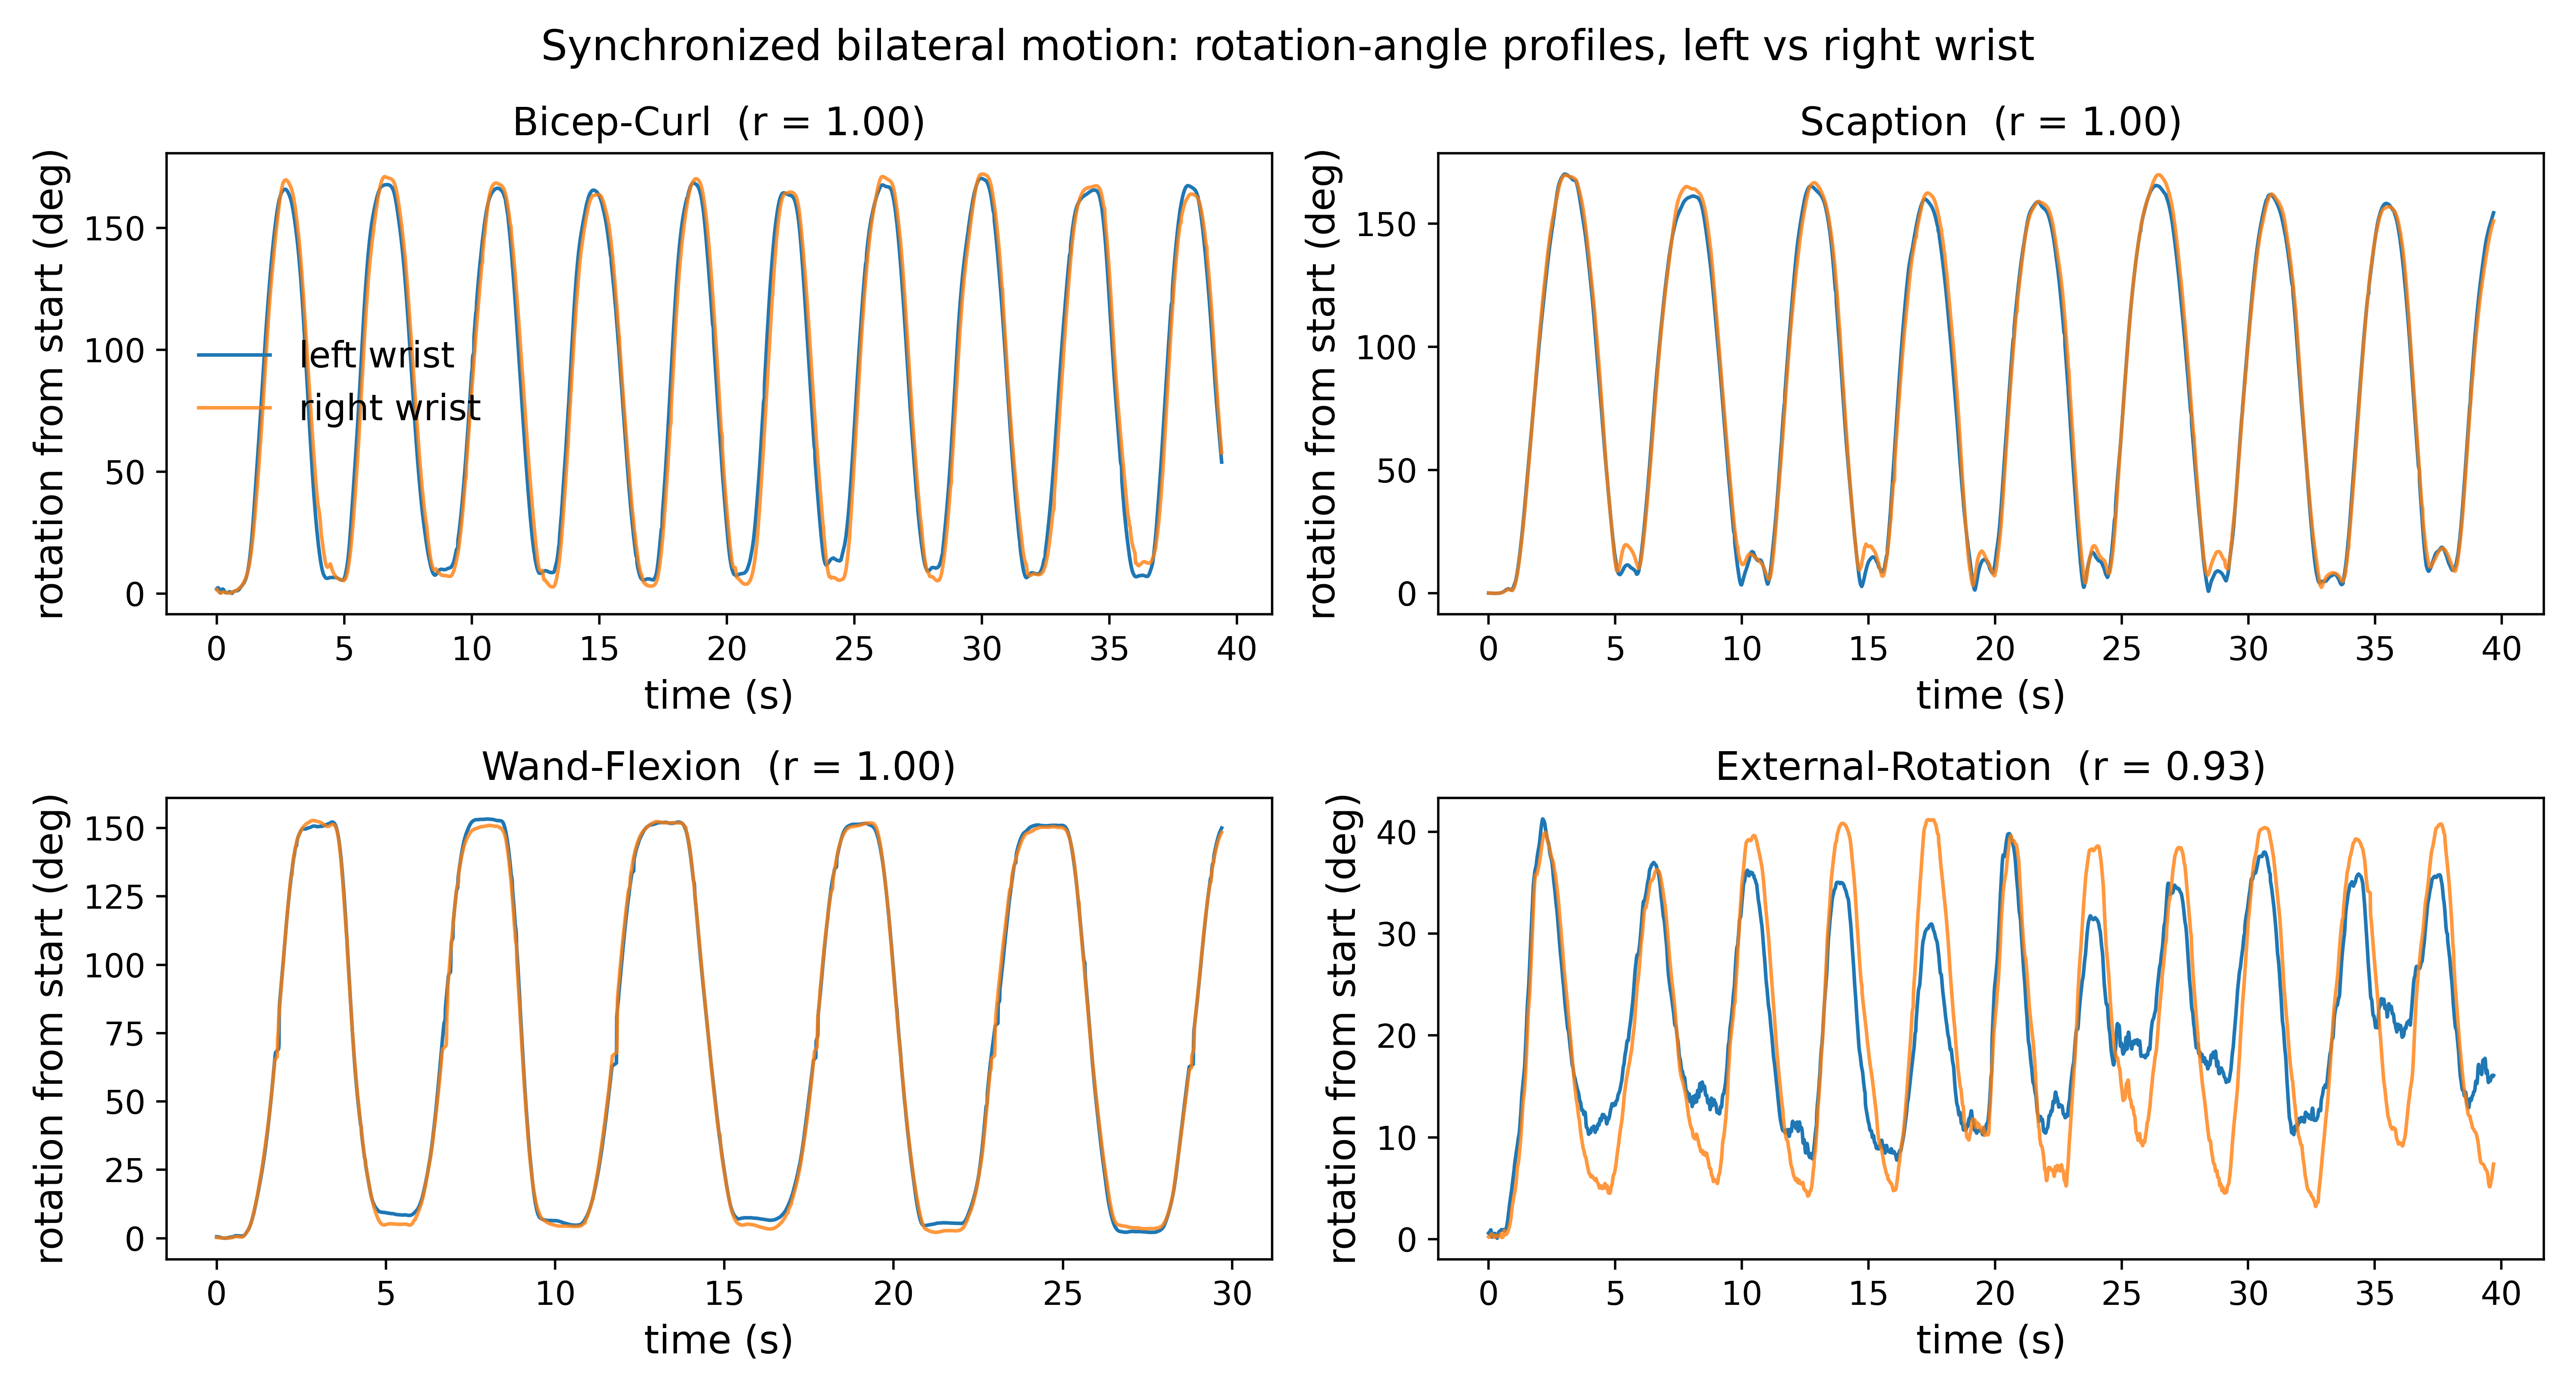
\includegraphics[width=\columnwidth]{figures/exp1_profiles.png}
\caption{Synchronized bilateral motion: frame-invariant rotation-angle
profiles of the left (blue) and right (orange) wrists during four
exercises of one subject.}
\label{fig:exp1}
\end{figure}

\subsection{Recognition and the cross-wrist gap (Experiments 2, 2b, 2c)}
The LOSO baseline reaches 92.1\% window and 93.7\% session accuracy
(macro-F1 0.916) over 12 classes and 8{,}187 windows
(Fig.~\ref{fig:exp2}); residual confusion concentrates among the three
small shoulder-elevation movements (lateral deltoid raise, scapular
retraction, front deltoid raise). Transferring across wrists without
correction collapses accuracy to 59.5\% (train right, test left) and
52.9\% (reverse). The estimated mirror map is physically coherent
(gravity $x$/$z$, roll, and gyro $y$ transfer directly; pitch, gravity
$y$, and gyro $x$/$z$ flip), and training on mirror-transformed data
restores 94.9--95.5\%. That this exceeds the within-wrist reference is
a property of the protocol, not evidence of leakage through the
transformation: at this stage the classifier trains on every subject's
source-wrist recordings, including those of the subject it is tested
on, whereas the within-wrist reference is leave-one-subject-out. The
mirrored condition uses exactly as many training windows as the raw
condition it is compared against --- only their signs differ --- so the
gain is attributable to the transformation rather than to training-set
size. The augmented condition does double the training set, and that
it matches the mirrored condition rather than exceeding it is further
evidence that the sign correction, not the added volume, is what
recovers the accuracy. Removing the subject overlap is precisely what
the next protocol does. Under the strictest protocol --- unseen subject
\emph{and} unseen wrist --- mirror-augmented training achieves
92.5--93.2\%, against a within-wrist reference of 92.9\%. That
reference is not the 92.1\% baseline above: it is computed on the
ten exercises recorded on both wrists and on the test wrist alone, so
it scores a slightly easier ten-class problem on matched test windows.
Because
``no worse than the reference'' is an equivalence claim rather than an
absence of difference, we test it as one (Experiment 2c): over the 22
paired subject folds the mean accuracy difference is $-0.02$ points
(90\% CI $[-1.0, +0.9]$), a paired Wilcoxon test finds no difference
($p = 0.99$), and two one-sided tests establish equivalence within a
pre-specified $\pm 2$-point margin ($p = 0.001$; $p = 0.033$ and
$p = 0.045$ for the two transfer directions separately). The
deployment gap is closed
(Fig.~\ref{fig:exp2b}).

\begin{figure}[t]
\centering
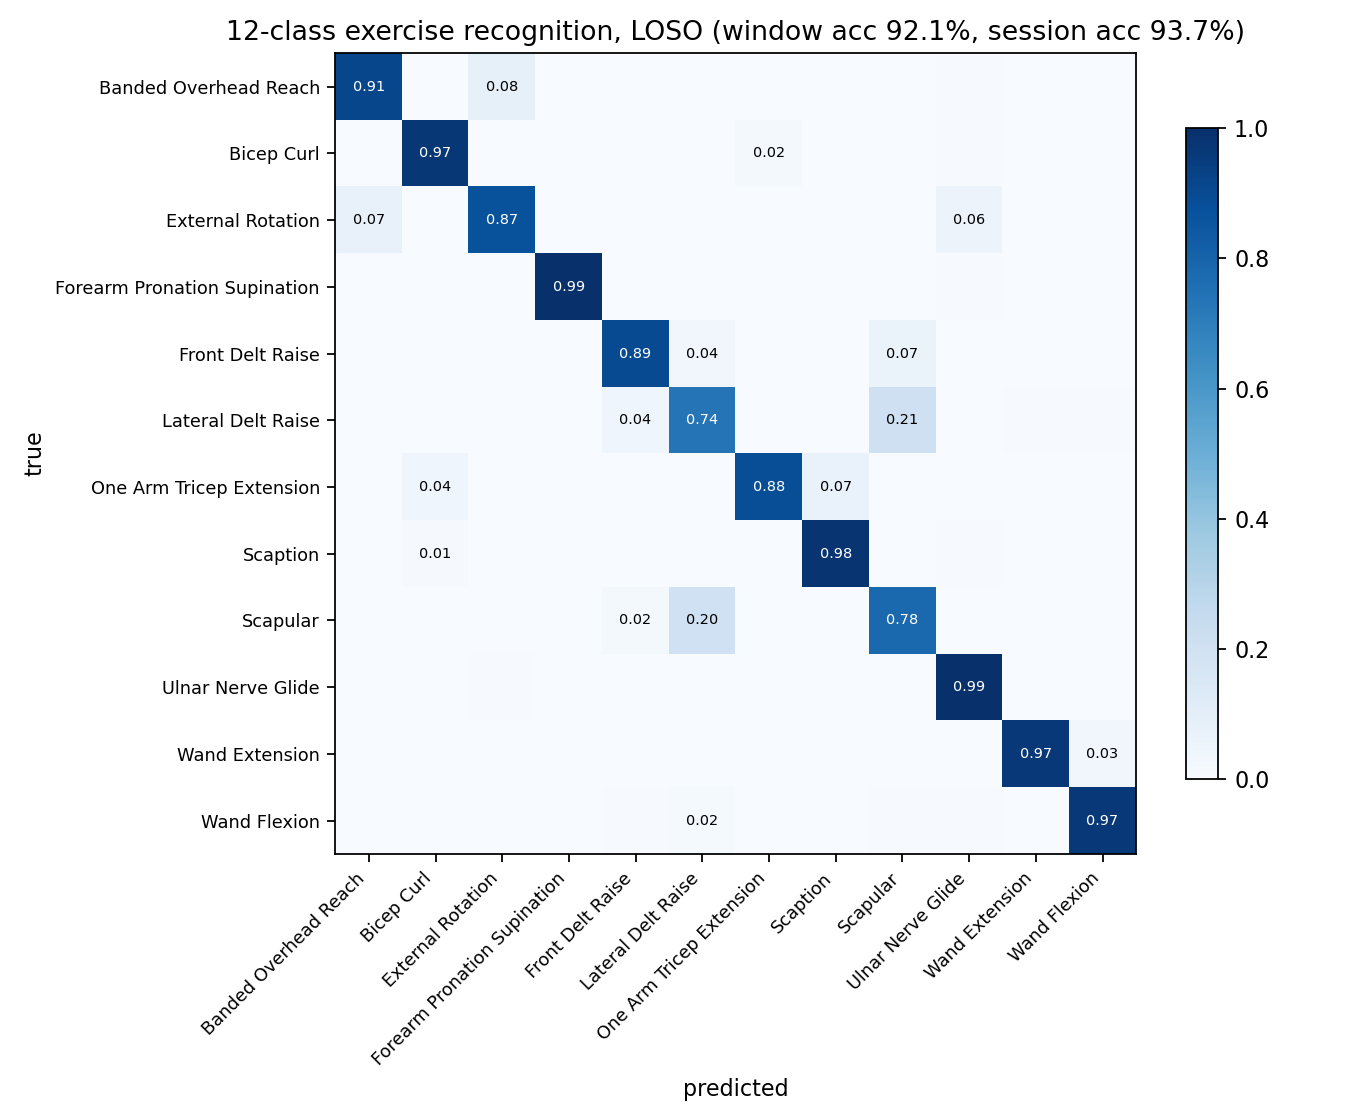
\includegraphics[width=\columnwidth]{figures/exp2_confusion.png}
\caption{12-class LOSO confusion matrix (window level, all folds).}
\label{fig:exp2}
\end{figure}

\begin{figure}[t]
\centering
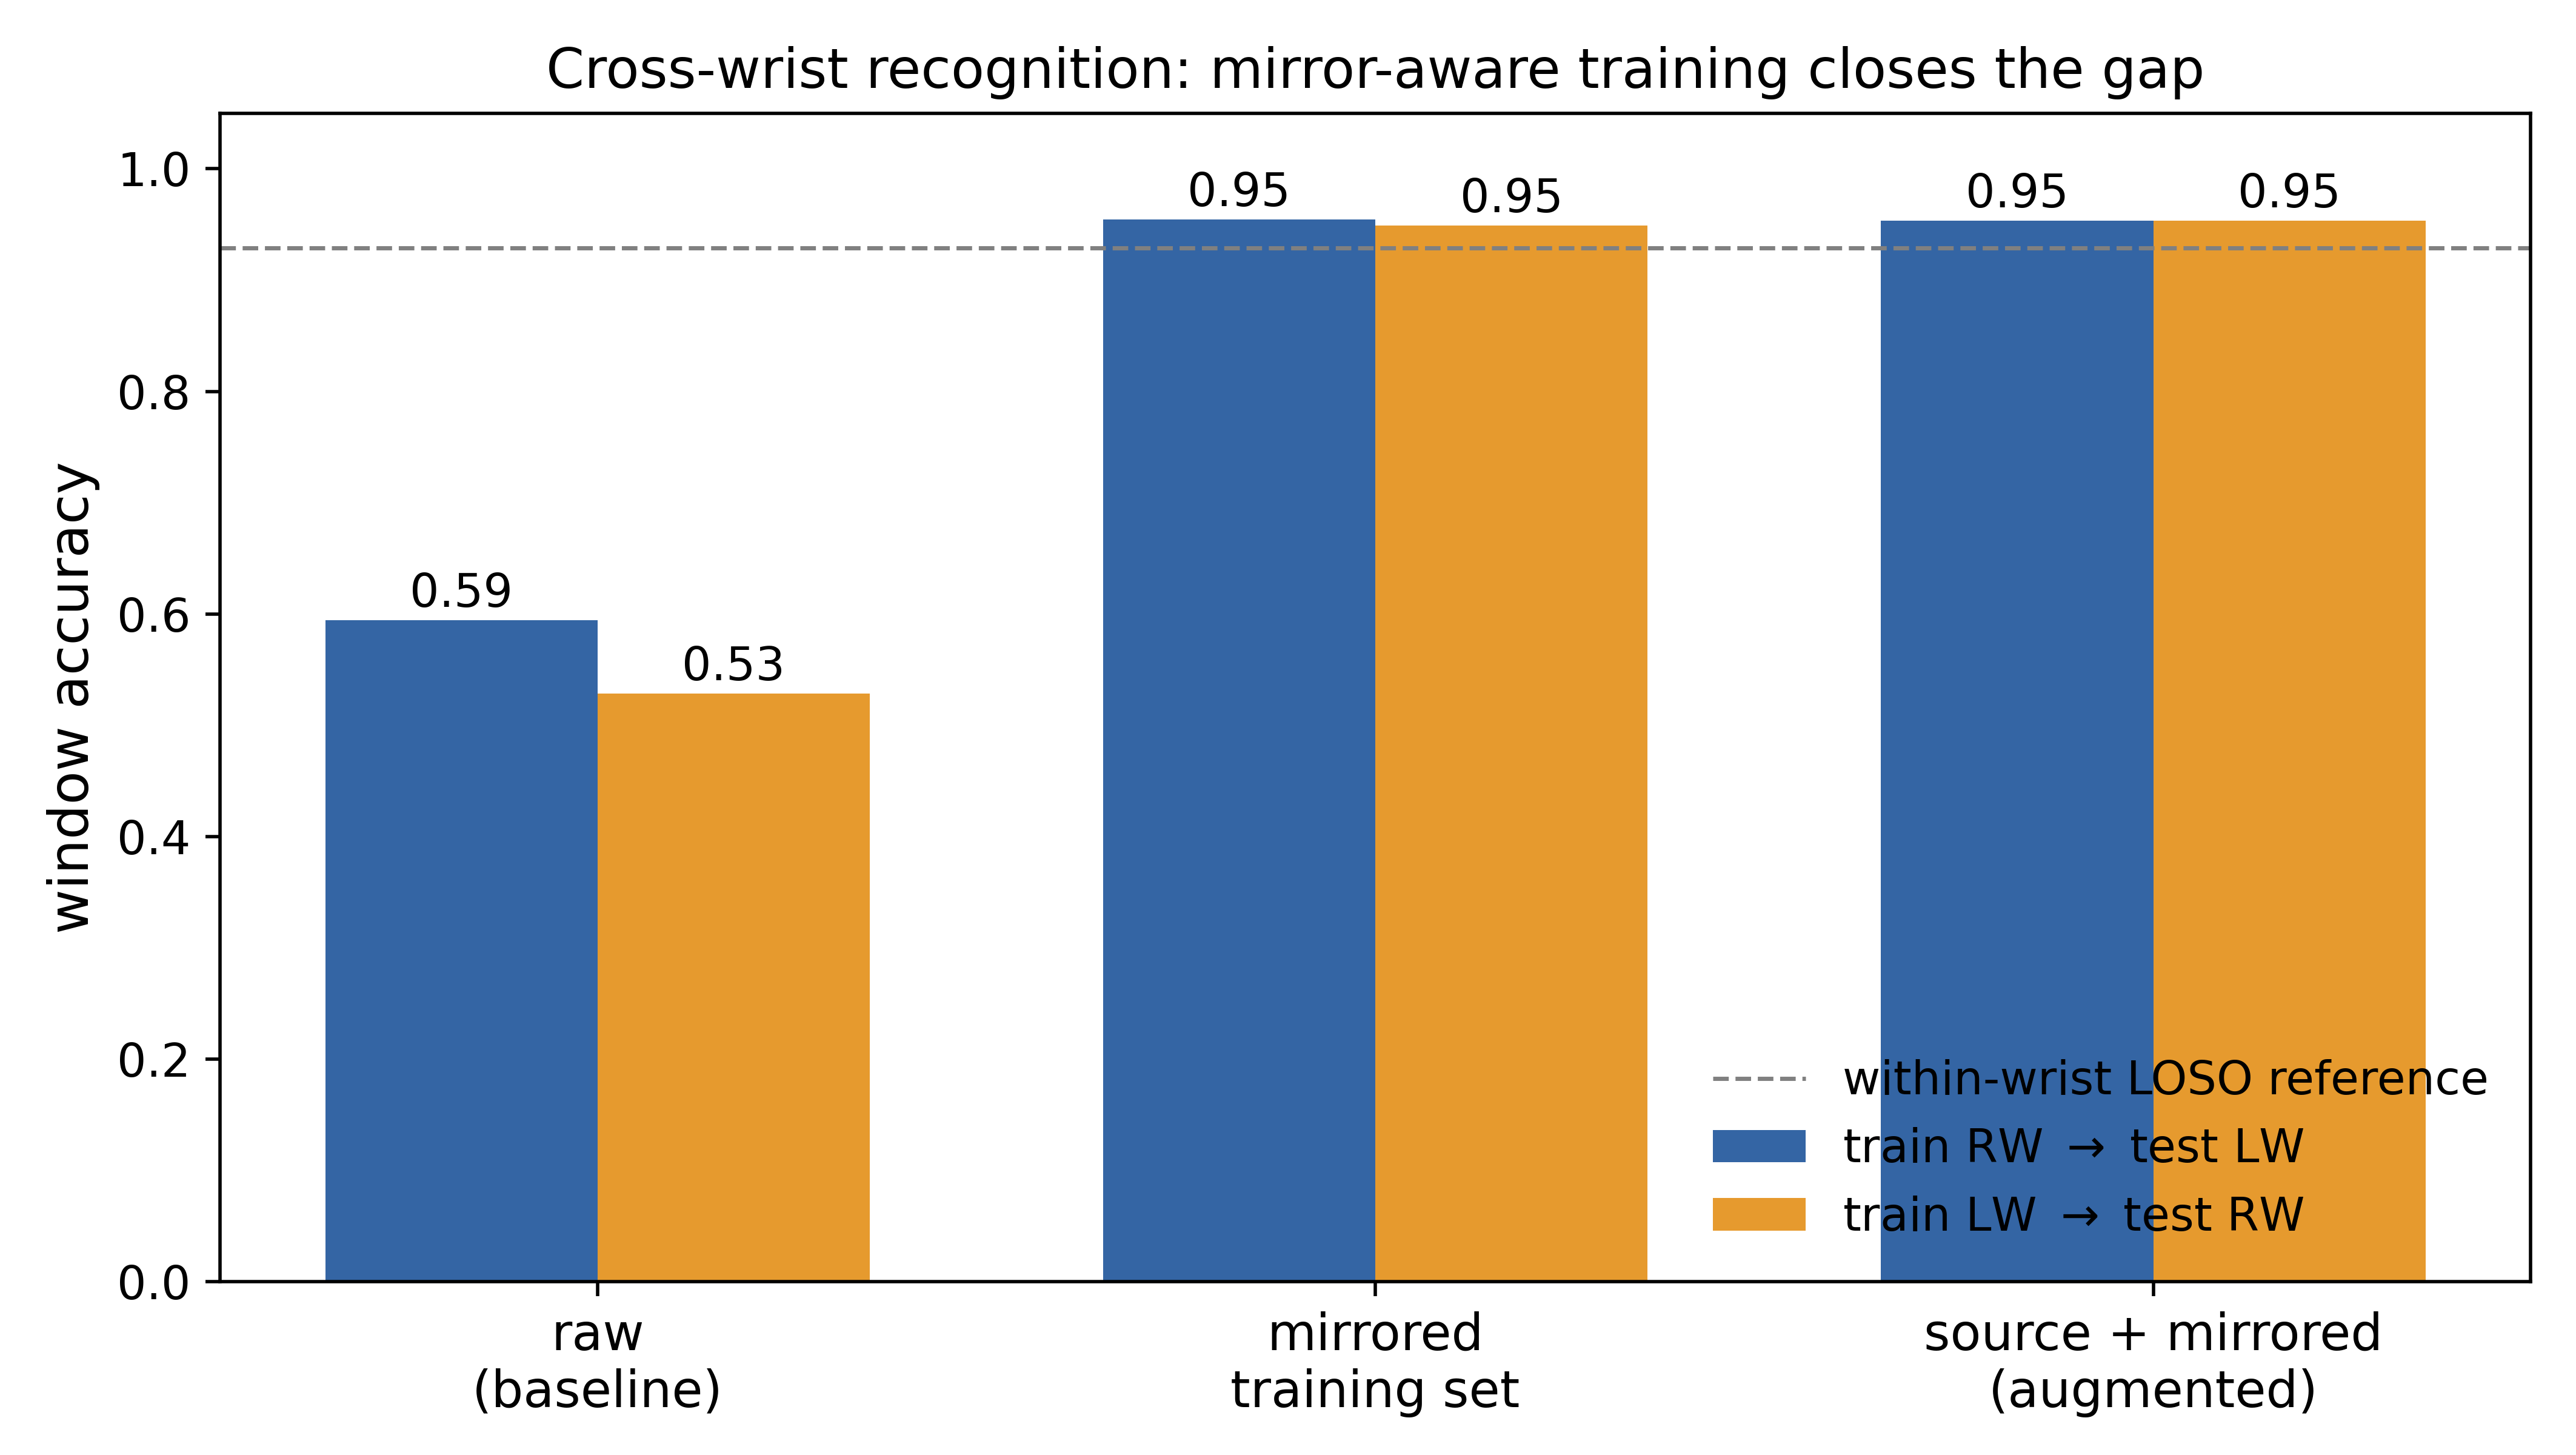
\includegraphics[width=\columnwidth]{figures/exp2b_gap.png}
\caption{Cross-wrist recognition with raw, mirrored, and augmented
training (wrist held out, subject not). The dashed line is the
within-wrist LOSO reference; the unseen-subject-and-unseen-wrist
results are reported in the text.}
\label{fig:exp2b}
\end{figure}

\subsection{Repetitions and motion primitives (Experiment 3)}
Segmentation yields 2{,}452 repetitions across 239 of 240 sessions;
in the remaining session no peak cleared the 40\%-prominence
threshold, so no repetition boundaries were emitted and the session
contributes no primitive.
Because the dual-wrist recordings observe the same physical movement,
per-wrist repetition counts validate each other: counts agree exactly
in 86.9\% of pairs and within $\pm 1$ in 94.4\%, with five of the six
larger disagreements again on external rotation. Per-exercise DMPs
reproduce their demonstrations with 0.5--1.7$^{\circ}$ median RMSE,
and the same primitive replays at scaled tempo and range
(Fig.~\ref{fig:exp3}) --- one demonstration yields a full difficulty
ladder.

\begin{figure}[t]
\centering
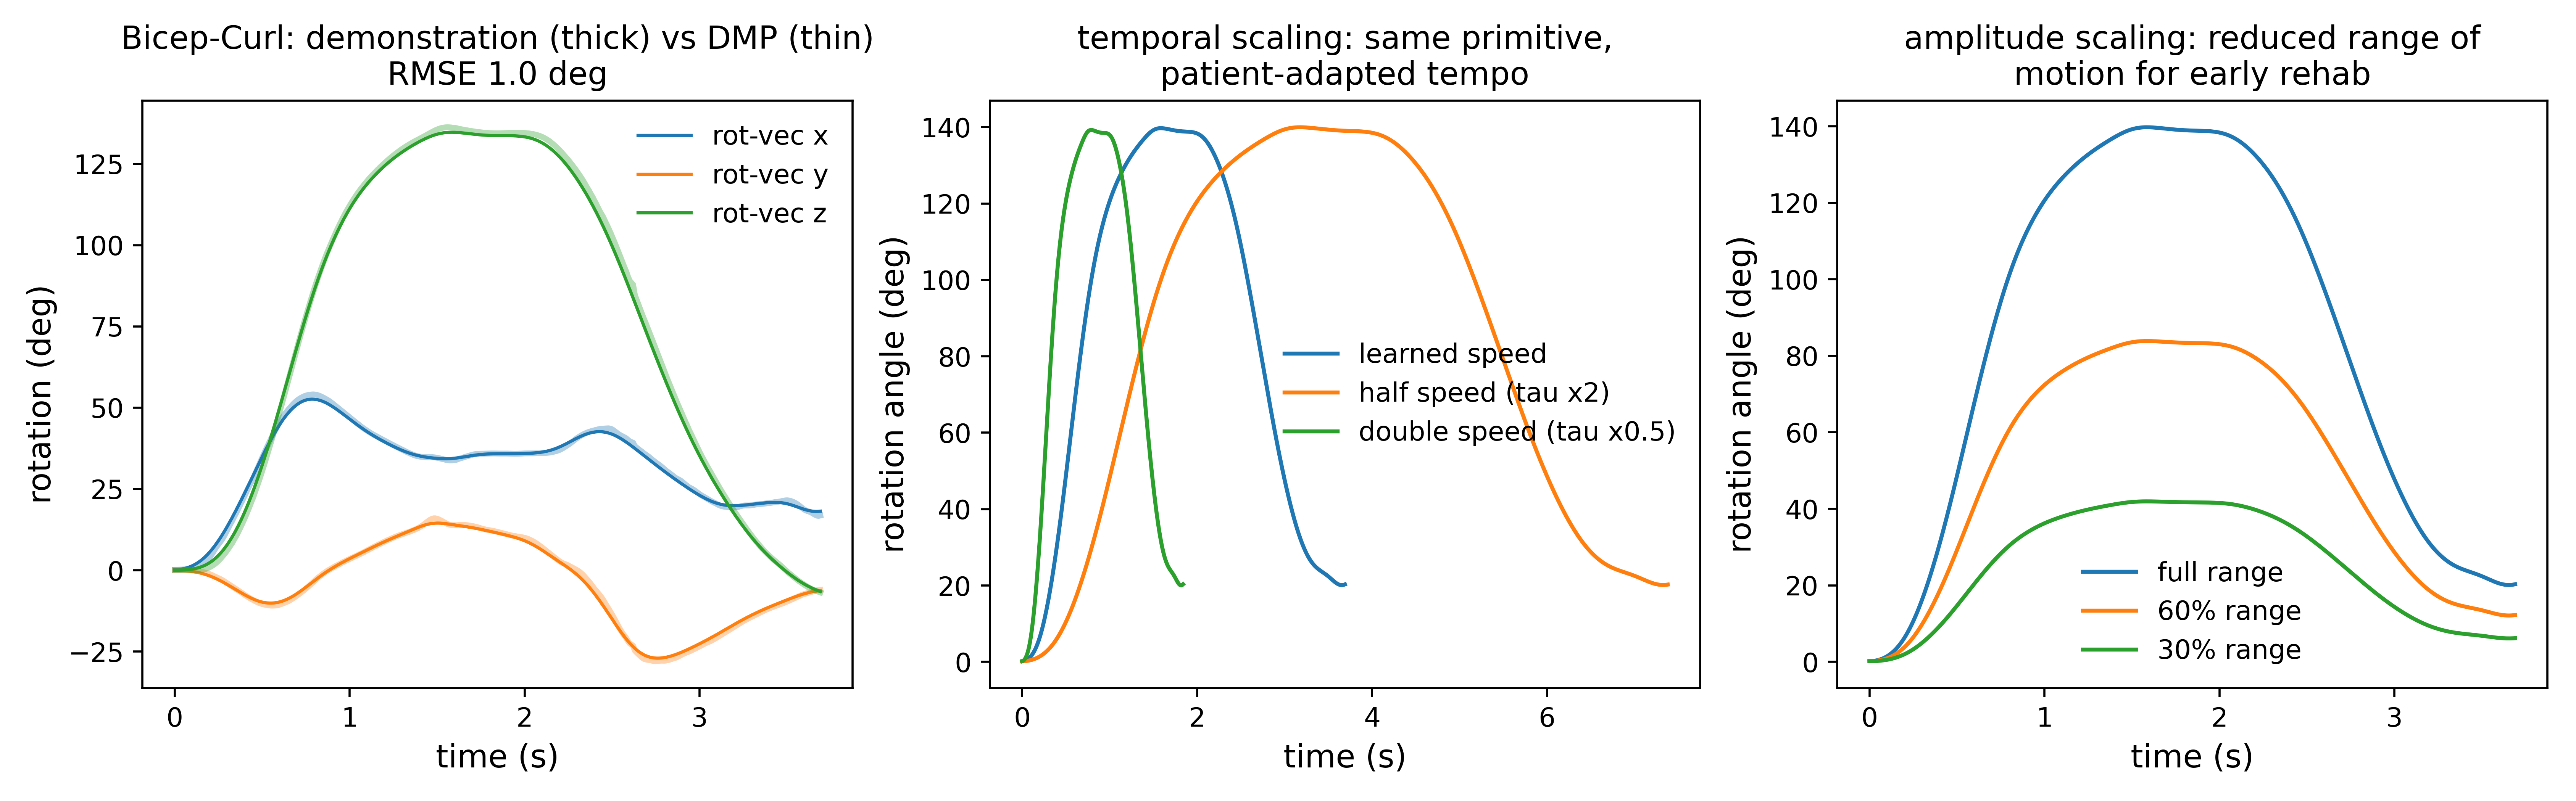
\includegraphics[width=\columnwidth]{figures/exp3_dmp.png}
\caption{Left: DMP reconstruction over the demonstration. Middle,
right: temporal and amplitude scaling of one learned primitive.}
\label{fig:exp3}
\end{figure}

\begin{figure}[t]
\centering
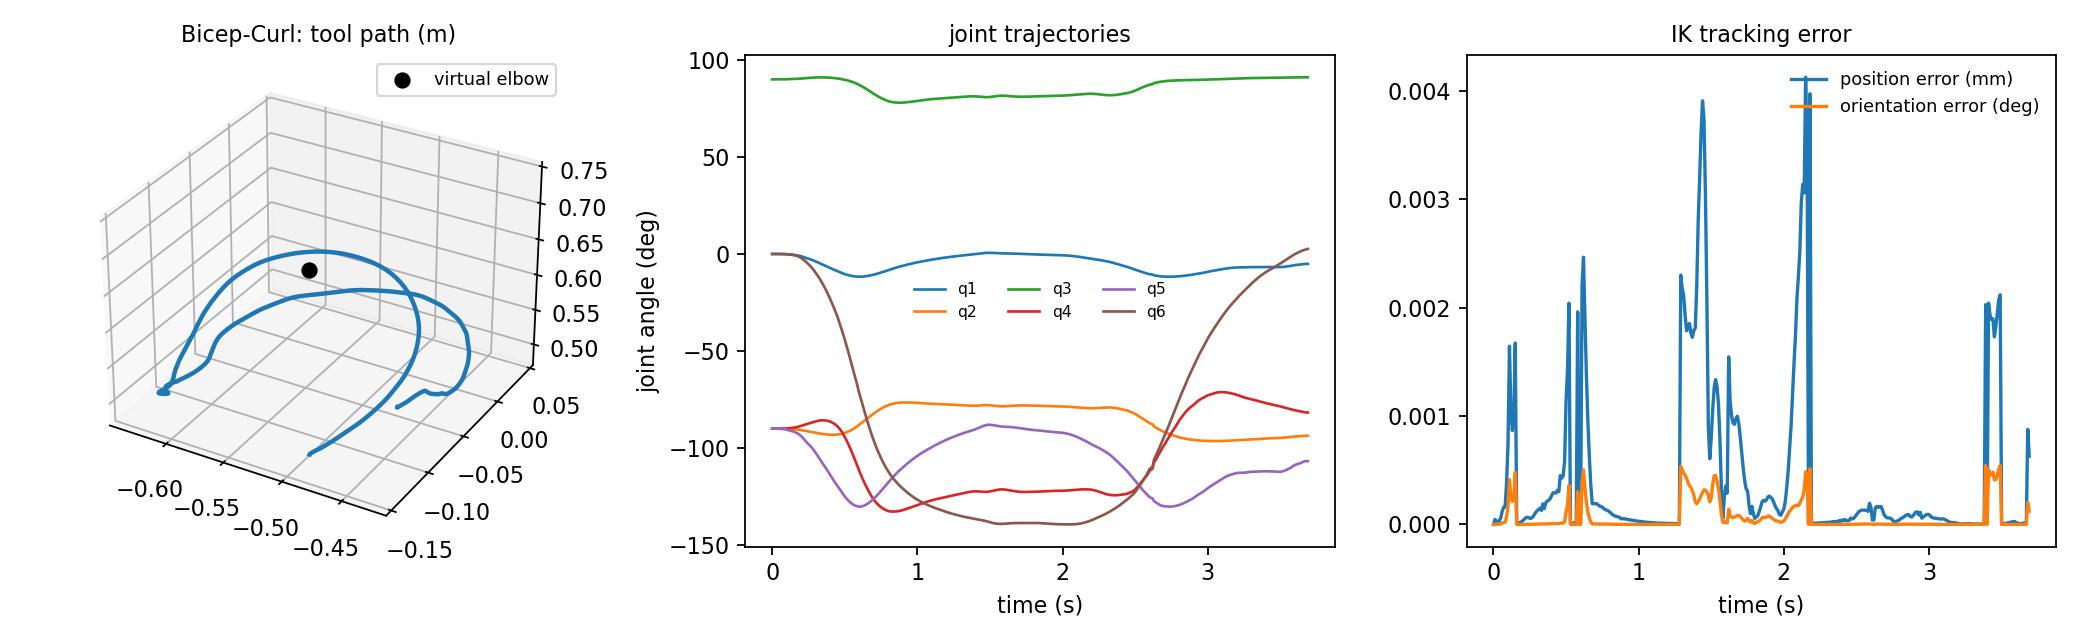
\includegraphics[width=\columnwidth]{figures/exp4a_retarget.png}
\caption{Retargeting one learned bicep-curl repetition to the UR5e.
Left: the commanded tool path traced about the virtual elbow anchor.
Middle: the six resulting joint trajectories. Right: inverse-kinematic
tracking error, which stays below 0.005~mm and 0.0006$^{\circ}$ for
this exercise.}
\label{fig:exp4a}
\end{figure}

\begin{figure}[t]
\centering
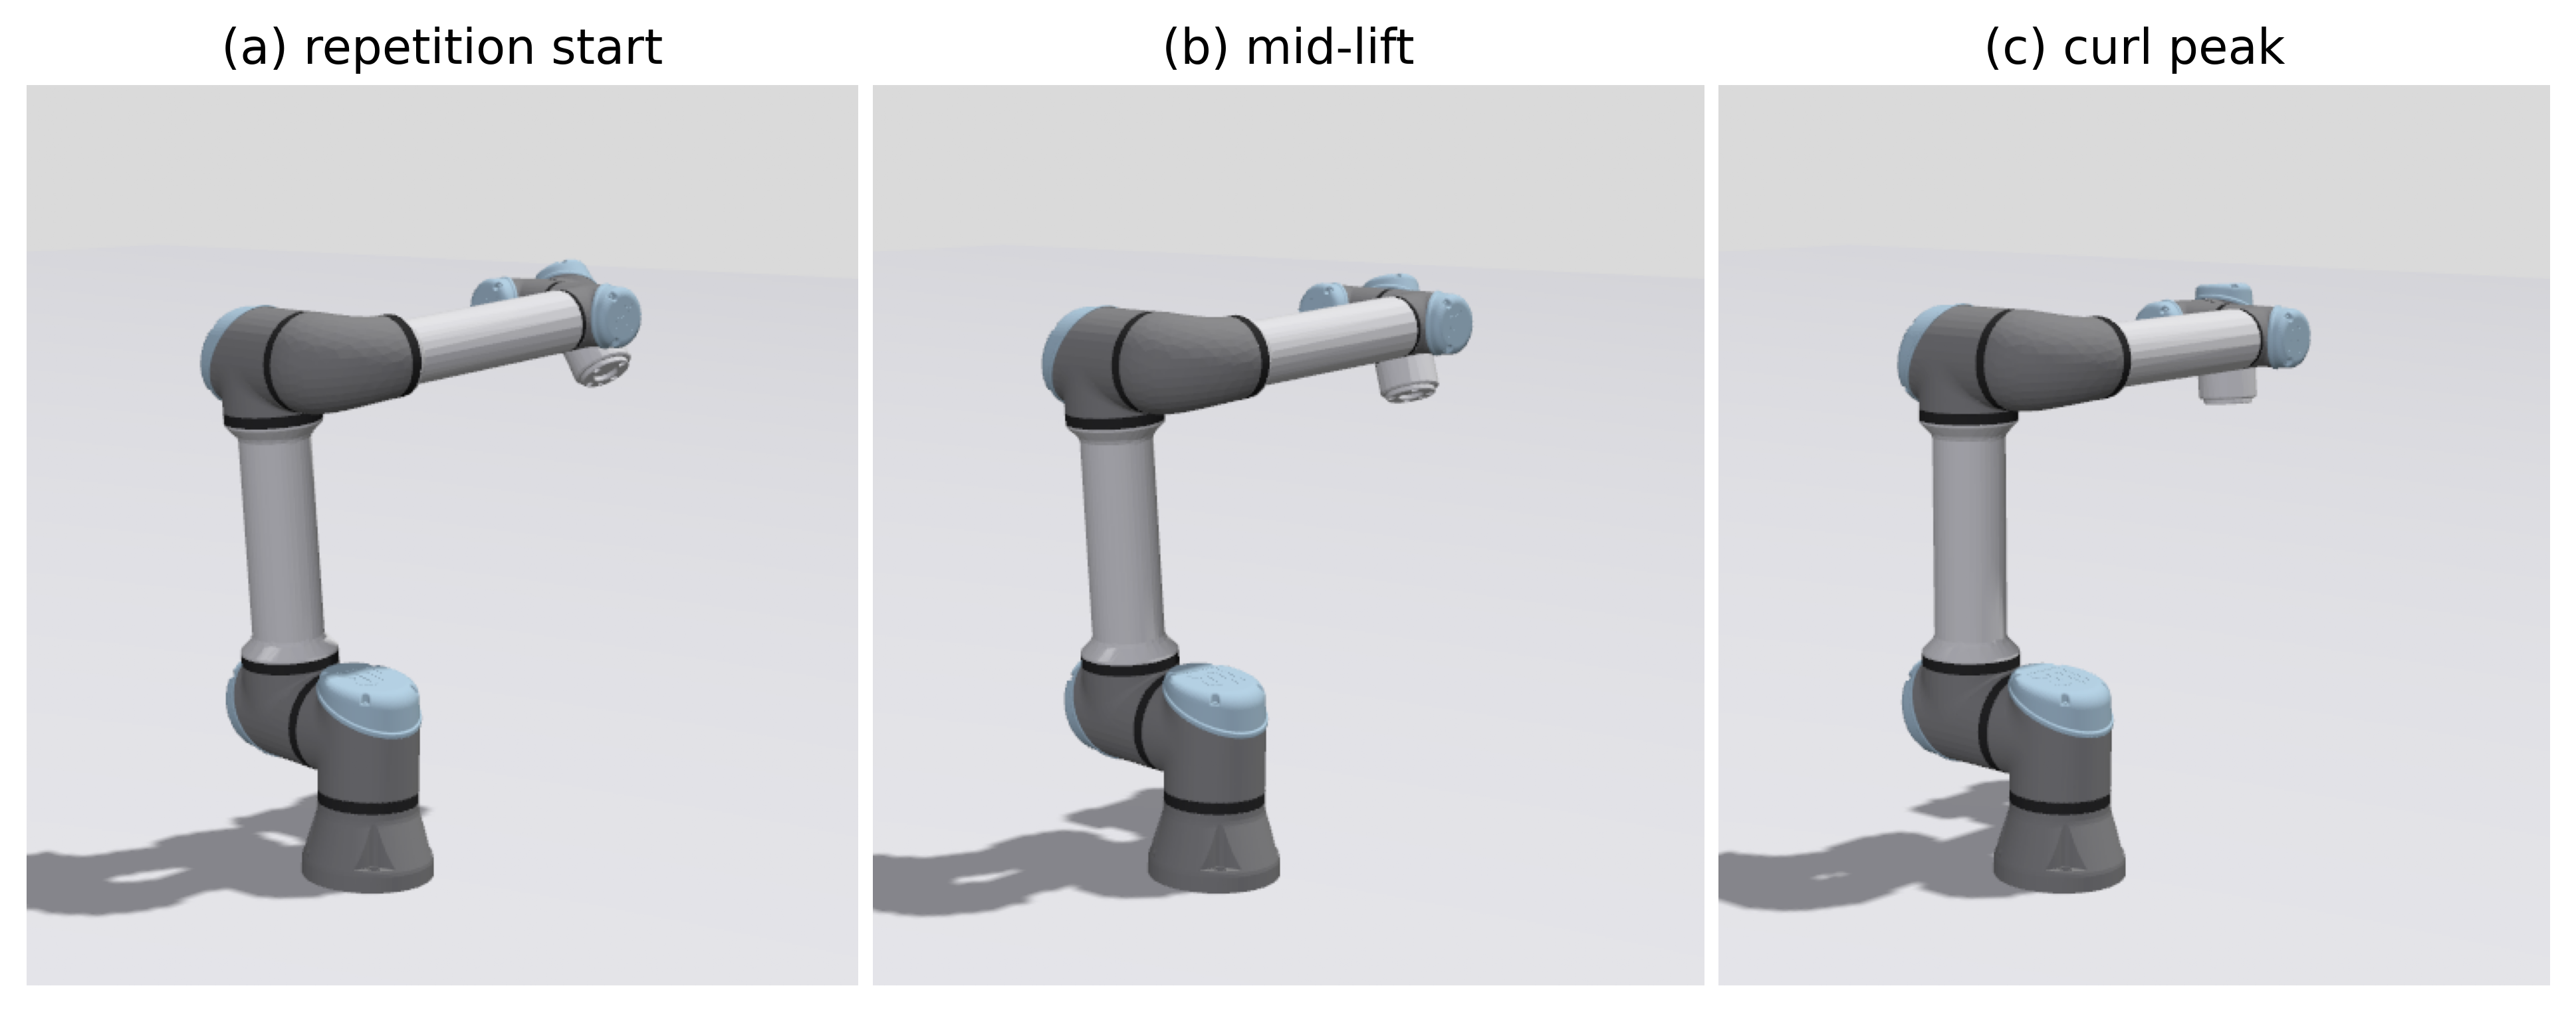
\includegraphics[width=\columnwidth]{figures/gazebo_exec.png}
\caption{The UR5e executing a learned Bicep-Curl primitive in Gazebo
(camera frames from the simulated therapy set). Under the single-pivot
retargeting, the exercise is carried by the tool's orientation: the
wrist sweeps the demonstrated hand arc from the hanging start pose (a)
through mid-lift (b) to the curl peak (c).}
\label{fig:gazebo}
\end{figure}

\subsection{Robot execution in simulation (Experiments 4a, 4b)}
All 12 retargeted exercises stay within UR5e joint limits and track
their pose references to better than 0.25$^{\circ}$ in orientation
(Fig.~\ref{fig:exp4a}).
Ten track to sub-millimeter position error; the exceptions are ulnar
nerve glide and wand flexion (18.6 and 19.8~mm peak), the same two
trajectories whose commanded joint velocities most exceed the arm's
limits at human tempo, where the step-capped IK solver lags the
reference at its fastest waypoints. Nine execute at demonstration
speed; forearm pronation--supination,
ulnar nerve glide, and wand flexion exceed wrist speed limits at human
tempo and require DMP time scaling of 2.05--3.02$\times$ --- the
primitive representation supplies exactly this knob. In Gazebo, all
12 exercises execute as five-repetition therapy sets with
0.07--0.56$^{\circ}$ mean joint tracking error
(Fig.~\ref{fig:gazebo}).


\subsection{Closed-loop verification in simulation (Experiment 4c)}
A random forest trained on all human windows classifies the
virtual-watch signals of the robot's executions correctly for
\textbf{10 of 12} exercises, most with 100\% window-vote agreement.
The two failures (front deltoid raise $\to$ scapular; lateral deltoid
raise $\to$ front deltoid raise) fall inside the classifier's known
human confusion cluster, amplified by the single-pivot retargeting
model, which most distorts translation-dominant raises. Two negative
results proved diagnostic: single-repetition executions were almost
universally misclassified (the features encode repetition rhythm),
and omitting the session's absolute reference attitude from the
virtual watch shifted every gravity-dependent feature, leaving only
2 of 12 exercises correctly recognized until the reference attitude
was restored.

\subsection{Movement-quality grading (Experiments 5, 5b)}
On 2{,}452 genuine repetitions (LOSO), the population envelope flags
healthy repetitions at 8.3\% while detecting injected tremor at 90\%,
truncation at 95\% (via end-point error), and half-range at 68\%.
Tempo faults evade it (23\%): healthy tempo varies more than
2$\times$ across people, so a population bound cannot represent
``too fast \emph{for you}''. The personalized envelope (own
calibration repetitions as center, quarter population width as floor)
lifts tempo detection to 66\% and half-range to 83\% at 7.7\% false
alarms --- a short supervised calibration session buys personalized
home grading (Fig.~\ref{fig:exp5}).

Executed on the robot (three exercises, five variants each), the
grader detects injected faults consistently with the offline study.
Tremor is flagged on 15 of 15 repetitions with \texttt{hf\_ratio}
among the named features; reduced range on 10 of 10 repetitions for the
two exercises with narrow population ROM spread (\texttt{rom\_deg}),
while wand extension's wide spread defeats the population bound ---
matching its offline rate. Clean executions are flagged on 5 of 15
repetitions --- four duration flags on lateral deltoid raise and one
end-point flag on bicep curl, with wand extension's clean set passing
entirely. This false-alarm rate exceeds the 8.3\% measured offline and
is a segmentation artifact of the robot protocol rather than a grader
failure: the inter-repetition return blend merges into the repetition
segment, inflating measured duration. Tightening the blend or
segmenting on the commanded trajectory would remove it. Over-speed programs are
caught \emph{before} grading: at full demonstration tempo the
trajectory controller aborts on path tolerance --- an execution-layer
safety net --- while over-speed inside tracking tolerance passes the
population envelope, consistent with the offline finding that tempo
faults require the personalized envelope. Truncated programs are not
flagged because they cannot physically occur in guided mode: the
protocol's return-to-start blend completes every repetition by design;
truncation remains detectable (95\%) for free-moving patients.

\begin{figure}[t]
\centering
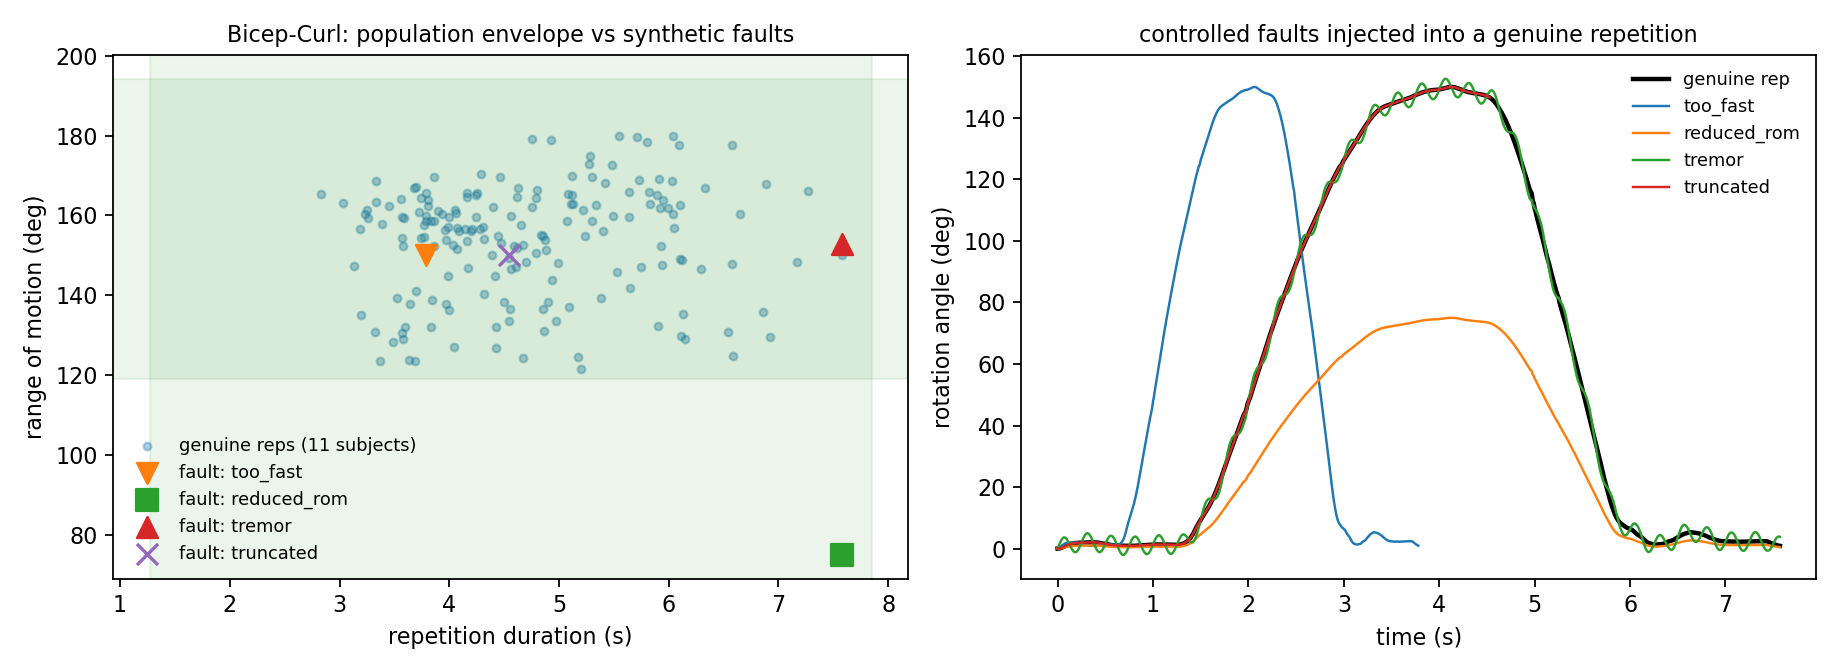
\includegraphics[width=\columnwidth]{figures/exp5_quality.png}
\caption{Left: population envelope (shaded) for one exercise with
fault positions of one repetition. Right: the injected fault types.}
\label{fig:exp5}
\end{figure}

\section{Discussion and Limitations}
\textbf{Scope.} We emphasize that every robot result in this paper is
\emph{simulation-based}: no physical robot was operated, and nothing
here constitutes physical-robot validation or clinical deployment.
Likewise, all subjects are healthy adults, and the movement faults of
Section~V-F are \emph{controlled synthetic injections} rather than
clinician-labelled patient errors --- detection rates on real
pathological movement may differ and require clinical data to
establish. The paper claims a validated pipeline, not a clinical
outcome. Future physical execution is intended to layer
admittance-controlled guidance over the collaborative arm's built-in
safety envelope --- enforced joint position and velocity limits (the
trajectories here already respect UR5e limits by construction),
reduced-speed mode, and a tool-center-point contact force limit on
the order of tens of newtons, well below injury thresholds --- so that
the software trajectory is bounded by hardware-enforced limits rather
than trusted alone. Any human--robot therapy additionally requires
ethics approval and a formal risk assessment; real human--robot
therapy remains future work.

\textbf{Wrist and device are confounded.} The protocol used the same
two physical watches throughout, one always worn on the left wrist and
the other always on the right (Section~III-B). Wrist side and device
identity are therefore perfectly collinear, and the raw cross-wrist
collapse we report may contain a device-specific component ---
unit-to-unit inertial bias, or differences in fit and mounting ---
alongside the anatomical mirroring the transformation is designed to
undo. The sign map is estimated from paired recordings and cannot
distinguish the two. Handedness is a second, weaker confound, as the
cohort is predominantly right-handed and exercises may be performed
differently with the dominant arm. Neither affects the deployment claim, which is
that a model trained on one wrist can be made to work on the other
under the conditions tested; both limit the anatomical interpretation.
Isolating them requires a device-swap subset --- the same subject
repeating an exercise with the two watches exchanged between wrists
--- which the present dataset does not contain and which we intend to
collect.

\textbf{The external-rotation thread.} The same exercise is the
outlier in mirror symmetry, repetition-count agreement, and (in human
data) recognition confusions: small-amplitude movements stress every
stage of a wrist-only pipeline. A second sensing modality or an upper
arm placement may be required for such exercises.

\textbf{Retargeting fidelity.} The single-pivot forearm model
reproduces hand orientation arcs faithfully but distorts
translation-dominant movements, which is visible as the two
verification failures. A richer target would add an estimated shoulder
joint center and a subject-scaled two-segment (upper-arm/forearm)
chain, and could fuse the watch's linear user-acceleration channel ---
unused here --- to constrain the hand's translational path rather than
its orientation alone. This is a natural next step precisely because
the failing exercises (deltoid raises) are the ones where hand
translation, not wrist orientation, carries the movement.

\textbf{Grading robot motion with human norms.} Idealized primitives
are \emph{smoother than any human}; a naive envelope flags them for
it. Clinically one-sided bounds (smoother-than-human is not a fault)
resolved this, a caution for anyone applying human-derived norms to
robot-mediated therapy.

\section{Conclusion}
A single consumer smartwatch can teach a physics-simulated rehabilitation robot a
12-exercise prescribed-exercise repertoire, verify its execution, and grade
movement quality --- with the left/right mirror assumption underpinning
wearable rehabilitation finally measured rather than assumed, and the
cross-wrist deployment gap it explains closed to within statistical
equivalence. These results are established on healthy volunteers and
on a physics simulation of the robot: they demonstrate that the
pipeline is technically sound end to end, and they are explicitly not
a clinical validation, which will require patient participants,
physical-robot execution, and clinician-labelled movement faults. The
dual-wrist dataset, all analysis code, and every figure in this paper
are reproducible from the public repository
(\url{https://github.com/Firaol-Tes/ASET_REHAB}).
Future work: execution on a physical UR5e, admittance-controlled
guidance, patient populations with clinical partners, and richer arm
models for translation-dominant exercises.

\section*{Data Availability}
All analysis code, experiment scripts, anonymized per-session results,
and the source of every figure and table in this paper are publicly
available at \url{https://github.com/Firaol-Tes/ASET_REHAB}.
The raw sensor recordings contain participant identifiers and are
available from the authors on reasonable request, subject to the
consent terms of the collection.

\section*{Acknowledgments}
The authors thank the volunteer subjects who contributed the
recordings, and the physiotherapists who advised on the exercise
protocol.

\begin{thebibliography}{9}
\bibitem{burns2018} D.~M. Burns \emph{et al.}, ``Shoulder
physiotherapy exercise recognition: machine learning the inertial
signals from a smartwatch,'' \emph{Physiological Measurement},
vol.~39, no.~7, 2018.
\bibitem{benachour2026review} Y.~Benachour \emph{et al.}, ``Machine
learning for wearable sensor-based human movement rehabilitation: A
five-year systematic review,'' \emph{IEEE Access}, vol.~14,
pp.~99280--99307, 2026, doi: 10.1109/ACCESS.2026.3707566.
\bibitem{krebs1998} H.~I. Krebs, N.~Hogan, M.~L. Aisen, and
B.~T. Volpe, ``Robot-aided neurorehabilitation,'' \emph{IEEE
Transactions on Rehabilitation Engineering}, vol.~6, no.~1,
pp.~75--87, 1998.
\bibitem{maciejasz2014} P.~Maciejasz \emph{et al.}, ``A survey on
robotic devices for upper limb rehabilitation,'' \emph{Journal of
NeuroEngineering and Rehabilitation}, vol.~11, no.~3, 2014.
\bibitem{ramachandran1996} V.~S. Ramachandran and D.~Rogers-Ramachandran,
``Synaesthesia in phantom limbs induced with mirrors,''
\emph{Proceedings of the Royal Society B}, vol.~263, pp.~377--386, 1996.
\bibitem{thieme2018} H.~Thieme \emph{et al.}, ``Mirror therapy for
improving motor function after stroke,'' \emph{Cochrane Database of
Systematic Reviews}, no.~7, 2018.
\bibitem{benachour2025} Y.~Benachour, M.~Rehman, and F.~Flitti,
``Towards improved human arm movement analysis: Advanced feature
engineering and model optimization,'' \emph{Engineering Applications
of Artificial Intelligence}, vol.~156, p.~111194, 2025.
\bibitem{araya2025} S.~T. Araya, S.~H. Eshetu, A.~M. Endale,
A.~A. Damtie, A.~B. Balcha, and M.~Rehman, ``Comparative analysis of
machine learning models for wearable rehabilitation movement
classification and on-device deployment feasibility,'' in \emph{Proc.
10th Int. Conf. on Information Technology Trends (ITT)}, Dubai, UAE,
2025, doi: 10.1109/ITT69610.2025.11352905.
\bibitem{eshetu2026} S.~H. Eshetu, S.~T. Araya, Y.~Benachour,
A.~B. Balcha, A.~A. Damtie, and A.~M. Endale, ``Hybrid CNN-LSTM
framework for upper-limb motion recognition using wearable IMU
sensors,'' in \emph{Proc. Int. Conf. on Interactive Systems \&
Information Society Technologies (InterSys)}, Dubai, UAE, 2026,
doi: 10.1109/InterSys69825.2026.11565250.
\bibitem{kedir2026} E.~M. Kedir, M.~A. Tilahun, G.~Bona, M.~Rehman,
F.~Flitti, and Y.~Benachour, ``Interpretable joint movement
classification via combinatorial DTW medoid distances and ensemble
feature selection,'' in \emph{Proc. Intelligent Information Systems
and Computing Conf. (IISCC)}, 2026.
\bibitem{bona2026} G.~Bona, M.~A. Tilahun, E.~M. Kedir, M.~Rehman,
F.~Flitti, and Y.~Benachour, ``Prototype-based DTW feature
representation for upper limb movement classification from
multichannel IMU signals,'' in \emph{Proc. Intelligent Information
Systems and Computing Conf. (IISCC)}, 2026.
\bibitem{bulling2014} A.~Bulling, U.~Blanke, and B.~Schiele, ``A
tutorial on human activity recognition using body-worn inertial
sensors,'' \emph{ACM Computing Surveys}, vol.~46, no.~3, 2014.
\bibitem{argall2009} B.~D. Argall, S.~Chernova, M.~Veloso, and
B.~Browning, ``A survey of robot learning from demonstration,''
\emph{Robotics and Autonomous Systems}, vol.~57, no.~5, pp.~469--483,
2009.
\bibitem{ijspeert2013} A.~J. Ijspeert \emph{et al.}, ``Dynamical
movement primitives: Learning attractor models for motor behaviors,''
\emph{Neural Computation}, vol.~25, no.~2, pp.~328--373, 2013.
\bibitem{balasubramanian2015} S.~Balasubramanian \emph{et al.}, ``On
the analysis of movement smoothness,'' \emph{Journal of
NeuroEngineering and Rehabilitation}, vol.~12, no.~112, 2015.
\bibitem{benachour2026ae} Y.~Benachour, A.~M. Endale, A.~B. Balcha,
A.~A. Damtie, S.~H. Eshetu, and S.~T. Araya, ``Hybrid multi-task LSTM
autoencoder for semantic anomaly diagnosis in rehabilitation
monitoring systems,'' in \emph{Proc. Int. Conf. on Communication,
Computing, Networking, and Control in Cyber-Physical Systems
(CCNCPS)}, 2026.
\end{thebibliography}

\end{document}
